\documentclass[12pt]{article}
\usepackage{amsmath, amssymb, amsthm}
\usepackage{geometry}
\usepackage{xcolor}
\usepackage{graphicx}
\geometry{margin=1in}

\title{Engineering Probability \\ Homework 4}
\author{Timothy Pollard, pollat@rpi.edu}
\date{October 1st 2025}

\begin{document}
\maketitle
\hrule

\section*{(1)}
The random variable $X$ has cumulative distribution function (CDF)
\[
F_X(x) =
\begin{cases}
0 & x < -3 \\
0.4 & -3 \leq x < 5 \\
0.8 & 5 \leq x < 7 \\
1 & x \geq 7
\end{cases}
\]

\begin{enumerate}
    \item[(a)] Sketch the graph of the CDF.
    \item[] 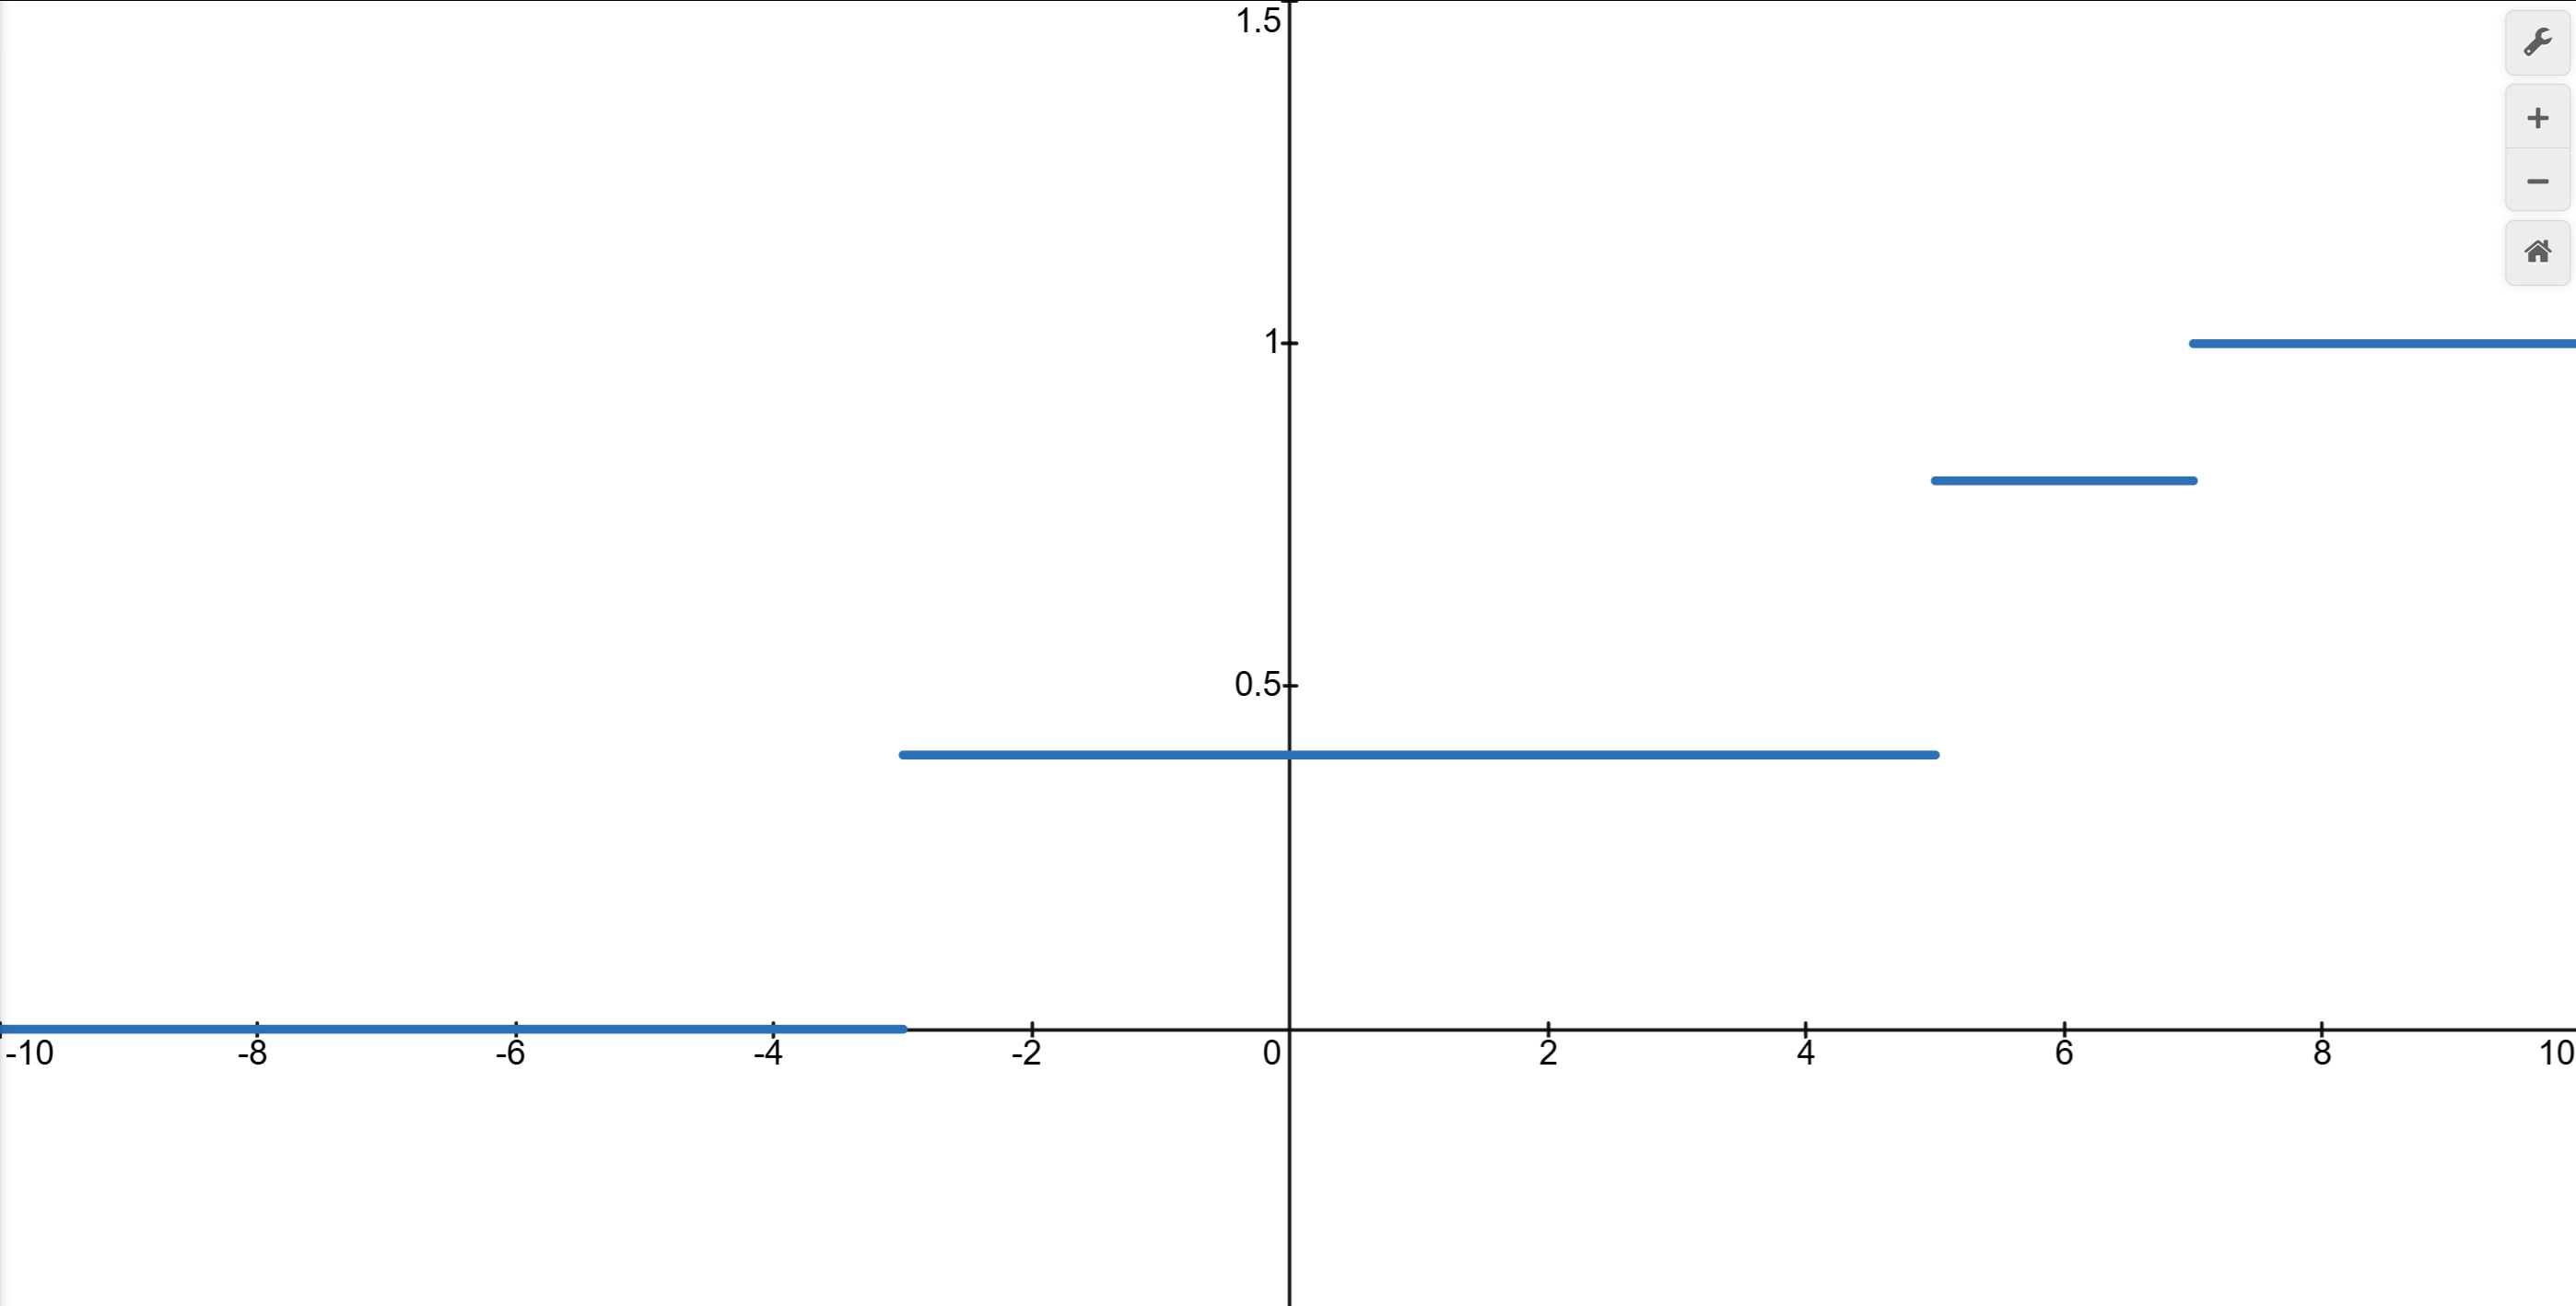
\includegraphics[width=0.5\textwidth]{CDF.png} 
    \item[(b)] Determine $P_X(x)$, the probability mass function (PMF) of $X$.
    \item[] \textcolor{blue}{\[
P_X(x) =
\begin{cases}
0.4 & x=-3,5 \\
0.2 & x = 7\\
0 & \text{otherwise}
\end{cases}
\]}
\newpage
    \item[(c)] Find the expected value, $E[X]$ of the random variable $X$.
    \item[] \textcolor{blue}{\[E[X] = \sum_{x\in S_X}^{}{x\cdot P_X(x)} = -3(0.4) + 5(0.4) + 7(0.2) = 2.2\]}
    \item[(d)] Find the variance, $\mathrm{Var}[X]$, of the random variable $X$.
    \item[] \textcolor{blue}{\[\mathrm{Var}[X] = E[X^2]- (E[X])^2 = \left((-3)^2(0.4) + (5)^2(0.4) + (7)^2(0.2)\right) -(2.2)^2 = 18.56\]}
\end{enumerate}

\section*{(2)}
At the One Top Pizza shop, a pizza sold has mushrooms with probability $p = \tfrac{2}{3}$. 
On a day in which 100 pizzas are sold, let $N$ be the number of pizzas sold before the first pizza with mushrooms is sold. What is the PMF of $N$? What is the CDF of $N$?

\textcolor{blue}{
\[
\text{PMF: } P_N(n) = 
\begin{cases}
\left(\frac{1}{3}\right)^n \left(\frac{2}{3}\right) & n = 0, 1, 2, \ldots \\
0 & \text{otherwise}
\end{cases}
\]
}

\textcolor{blue}{
\[
\text{CDF: } F_N(n) =
\begin{cases}
 1 - \left(\frac{1}{3}\right)^{n+1}& n = 0, 1, 2, \ldots\\
0 & \text{otherwise}
\end{cases}
\]}

\section*{(3)}
Let $X$ have the uniform PMF
\[
P_X(x) =
\begin{cases}
0.01 & x = 1, 2, \ldots, 100 \\
0 & \text{otherwise}
\end{cases}
\]

\begin{enumerate}
    \item[(a)] Find a mode $x_{\text{mod}}$ of $X$. If the mode is not unique, find the set $X_{\text{mod}}$ of all modes of $X$.
    \item[] \textcolor{blue}{The mode is not unique b/c it's a uniform PMF, $X_{\text{mod}} = \{1, 2, \ldots, 100\}$.}
    \item[(b)] Find a median $x_{\text{med}}$ of $X$. If the median is not unique, find the set $X_{\text{med}}$ of all numbers $x$ that are medians of $X$.
    \item[] \textcolor{blue}{$x_{med} = \{50,51\}$}
\end{enumerate}
\newpage

\section*{(4)}
Voice calls cost 20 cents each and data calls cost 30 cents each. $C$ is the cost of one telephone call. The probability that a call is a voice call is $P[V] = 0.6$. The probability of a data call is $P[D] = 0.4$.

\begin{enumerate}
    \item[(a)] Determine $P_C(c)$, the PMF of $C$.
    \item[] \textcolor{blue}{\[
P_C(c) =
\begin{cases}
0.6 & c = 20 \\
0.4 & c = 30 \\
0 & \text{otherwise}
\end{cases}
\]}
    \item[(b)] Determine $E[C]$, the expected value of $C$.
    \item[] \textcolor{blue}{\[E[C] = 20(0.6) + 30(0.4) = 24\]}
    \item[(c)] Determine $\mathrm{Var}[C]$, the variance of $C$.
    \item[] \textcolor{blue}{\[\mathrm{Var}[C] = E[(C-\mu_X)^2] = \sum_{c\in S_C}^{}{(c-\mu)^2\cdot P_C(c)} = (20-24)^2(0.6) + (30-24)^2(0.4) = 24\]}
    
\end{enumerate}
\newpage

\section*{(5)}
Given the random variable $X$ in Problem 1, let $W = g(X) = -X$.

\begin{enumerate}
    \item[(a)] Determine $P_W(w)$.
    \item[] \textcolor{blue}{\[
P_W(w) =
\begin{cases}
0.4 & w=3,-5 \\
0.2 & w = -7\\
0 & \text{otherwise}
\end{cases}
\]}
    \item[(b)] Determine $F_W(w)$.
    \item[] \textcolor{blue}{ \[
F_W(w) =
\begin{cases}
0 & w < -7 \\
0.2 & -7 \leq w < -5 \\
0.6 & -5 \leq w < 3 \\
1 &  w \geq 3
\end{cases}
\]}
    \item[(c)] Determine $E[W]$.
    \item[] \textcolor{blue}{\[E[W]=\sum_{x\in S_X}^{}{-x\cdot P_X(x)} =-E[X]= -2.2\]}
    \item[(d)] Determine $\mathrm{Var}[W]$.
    \item[] \textcolor{blue}{\[\mathrm{Var}[W] = (-1)^2\mathrm{Var}[X] = 18.56\]}
\end{enumerate}
\newpage 

\section*{(6)}
At a discount brokerage, a stock purchase or sale worth less than \$10{,}000 incurs a brokerage fee of 1\% of the value of the transaction. A transaction worth more than \$10{,}000 incurs a fee of \$100 plus 0.5\% of the amount exceeding \$10{,}000. Note that for a fraction of a cent, the brokerage always charges the customer a full penny. You wish to buy 100 shares of a stock whose price $D$ in dollars has a PMF

\[
P_D(d) =
\begin{cases}
\tfrac{1}{3} & d = 99.75,\, 100,\, 100.25 \\
0 & \text{otherwise}
\end{cases}
\]

What is the PMF of $C$, the cost of buying stock (including brokerage fee).
\textcolor{blue}{
\[
d = 99.75, 100, 100.25
\]
\[
c_{99.75} = 9,975 + (9975\cdot 1\%) = 10,074.75
\]
\[
c_{100} = 10,000 + (10,000\cdot 1\%) = 10,100
\]
\[
c_{100.25} = 10,025 + (100+ 25\cdot0.5\%) = 10,125.13 \text{ (rounded up)}
\]
\[
P_C(c) =
\begin{cases}
\tfrac{1}{3} & c = 10074.75,\, 10100,\, 10125.13 \\
0 & \text{otherwise}
\end{cases}
\]
}

\section*{(7)}
Let $X$ be a discrete random variable with PMF
\[
P_X(x) =
\begin{cases}
\tfrac{1}{8}, & x = 1, 2, 3, 4, \\[6pt]
\tfrac{1}{2}, & x = 5, \\[6pt]
0, & \text{otherwise}.
\end{cases}
\]

Define a new random variable
\[
Y = g(X) =
\begin{cases}
0, & x \in \{1, 2\}, \\
1, & x \in \{3, 4, 5\}.
\end{cases}
\]

\begin{enumerate}
    \item[(a)] Determine the PMF of $Y$.
    \item[] \textcolor{blue}{\[P_Y(y) =
\begin{cases}
\frac{1}{4}, & y = 0, \\[6pt]
\frac{3}{4}, & y = 1, \\[6pt]
0, & \text{otherwise}.
\end{cases}
\]}
    \item[(b)] Derive the CDF of $Y$.
    \item[] \textcolor{blue}{\[F_Y(y) =
\begin{cases}
0, & y < 0, \\[6pt] 
\frac{1}{4}, & 0 \leq y < 1, \\[6pt]
1, & y \geq 1.
\end{cases}
\]}
    \item[(c)] Compute the expected value $E[Y]$.
    \item[] \textcolor{blue}{\[E[Y] = 0\left(\frac{1}{4}\right) + 1\left(\frac{3}{4}\right) = \frac{3}{4}\]}
    \item[(d)] Determine the variance $\mathrm{Var}[Y]$ and the standard deviation of $Y$.
    \item[] \textcolor{blue}{\[\mathrm{Var}[Y] = E[Y^2] - (E[Y])^2 = 0^2\left(\frac{1}{4}\right) + 1^2\left(\frac{3}{4}\right) - \left(\frac{3}{4}\right)^2 = \frac{3}{16}\]}
\end{enumerate}

\end{document}

